% Waterfall chart: decode kernel cumulative instret reduction per tier
% Chapter 8 - HQC-128 Decaps decode kernel, Spike ISS
% Data source (commit bdd9cf4, 2026-06-30): sim_decode_128_latest.csv
%   Reference : scalar        = 1,052,692
%   +Zbc      : Tier 1 scalar =   604,218  (1.74x)
%   +base-RVV : Tier 2        =   134,737  (7.81x)
%   +Zvbc     : Tier 3        =    73,769  (14.27x)
% IMPORTANT: symbolic x coords must be PLAIN TEXT (no \Zbc / \RVV macros).
% Those macros expand to \ext{..}\xspace (= \textsf{..}\xspace); when combined
% with `nodes near coords', pgfplots feeds the stored coordinate token list
% into its per-point handler, which trips an xcolor \XC@definec@lor error and
% aborts the picture mid-way. House style: see kem-breakdown-stacked.tex.
\tikzsetnextfilename{ch8-results-decode-waterfall}
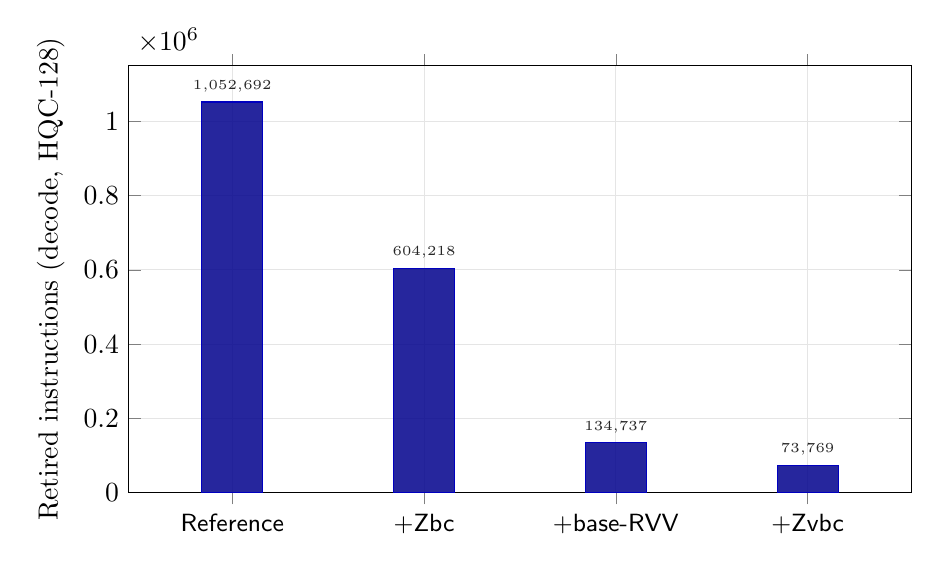
\begin{tikzpicture}
\begin{axis}[
    ybar,
    bar width=22pt,
    width=0.95\textwidth,
    height=7cm,
    ylabel={Retired instructions (decode, HQC-128)},
    symbolic x coords={Reference, +Zbc, +base-RVV, +Zvbc},
    xtick=data,
    x tick label style={font=\sffamily\small},
    ymin=0,
    ymax=1150000,
    scaled y ticks=base 10:-6,
    ytick scale label code/.code={$\times 10^6$},
    nodes near coords,
    nodes near coords style={font=\tiny, /pgf/number format/fixed},
    every axis plot/.append style={fill opacity=0.85},
    grid=major,
    grid style={gray!20},
    enlarge x limits=0.18,
]

\addplot[fill=blue!55!black, draw=blue!75!black] coordinates {
    (Reference,   1052692)
    (+Zbc,         604218)
    (+base-RVV,    134737)
    (+Zvbc,         73769)
};

\end{axis}
\end{tikzpicture}
